\section{Tutorial}
\label{tutorial_csp}

The objective of this chapter is to get you to a stage where you can use BMotion Studio to visualize CSP-M models. 
We expect that you have already downloaded the BMotion Studio tool (see Section~\ref{installation}) and created a new visualisation template for Event-B visualisations (see Section~\ref{vis_template}).
 
%We expect you to have a basic understanding of logic and an idea why doing formal modelling is a good idea.  
You should be able to work through the tutorial with no or little outside help.

We encourage you not to download solutions to the examples but instead to actively build them up yourself as the tutorial progresses.

If something is unclear, remember to check the Reference (\ref{reference_csp}) for more information.

\subsection{Creating a new Visualisation Template}

Let's start by creating a new visualisation template.
The easiest way to create a new visualisation template is to duplicate the default template \texttt{csp\_template} that is included in the \texttt{workspace} folder of your \bms~installation.
Just duplicate the \texttt{csp\_template} folder and rename it to \texttt{bully}.
After refreshing your browser, a new folder called \texttt{bully} should appear in your workspace.

\subsection{The Formal Model}

We are going to create a visualisation of the bully algorithm specification found in the book ``Understanding Concurrent Systems'' (ISBN 978-1-84882-258-0).
The algorithm represents a method of distributed computing for electing a node to be the coordinator amongst a group of nodes.
Each node has a unique ID and the algorithm intends to select the node with the highest ID to be the coordinator.
It is assumed that the nodes may fail and revive from time to time and the communication between the nodes is reliable.
Three types of messages are defined within the design of the algorithm: \textit{election} (announcing an election), \textit{answer} (responding to an election message), and \textit{coordinator} (announcing the identity of the coordinator).

You can download the CSP model \file{BullyAlgorithm.zip}{here}.
Decompress it and put the files into a new folder called \texttt{model} relative to your \texttt{template.html} file in your workspace.

\subsection{Linking a Model with the Visualisation}

The next step consists of linking the model with the visualisation.
For this, open the \texttt{template.html} file with an HTML/text editor of your choice and add the following line within the head tag:

\begin{lstlisting}[language=html]
<meta name="bms.model" content="model/bully.csp" />
\end{lstlisting}

We link the visualisation with the CSP-M model called ``bully.csp''.
Linking a model within the \texttt{template.html} file automatically loads the model, when starting the visualisation.
Your \texttt{template.html} file should look like:

\begin{lstlisting}[language=html]
<html bms-app>
  <head>
      <title>BMotion Studio for ProB</title>
      <meta name="bms.model" content="model/bully.csp" />
      <meta name="bms.tool" content="CSPAnimation" />
      <meta name="bms.script" content="template.groovy" />
      <script src="/bms/libs/requirejs/require.js"></script>
      <script>
        require(['/bms/libs/prob/config.js'], function () {
          require(['template']);
        });
      </script>
  </head>
  <body>
  </body>
</html>
\end{lstlisting}

\info{The meta tag \textit{bms.script} (line 6) contains the link to the Groovy script file and the meta tag \textit{bms.tool} (line 5) defines the formalism or the simulator respectively that should be used. In this case we are creating a visualisation for a ``CSPAnimation'' (CSP models).}

\subsection{Creating the Actual Visualisation}

The next step consists of creating the actual visualisation.
The user is not restricted to an editor in order to create a visualisation.
The user can make use of any tool that support the creation of SVG graphics or HTML documents.
For this tutorial we are going to use the Inkspace\footnote{\url{https://inkscape.org}} editor. Inkscape is an editor for creating vector graphics that is available for Windows, Mac OS X and Linux.
It's free and open source.
With Inkscape the user can export the vector graphic into the SVG format.

%\info{We are currently working on a build-in graphical editor for creating SVG graphics and for managing observers.}

\begin{figure}[!ht]
\begin{center}
	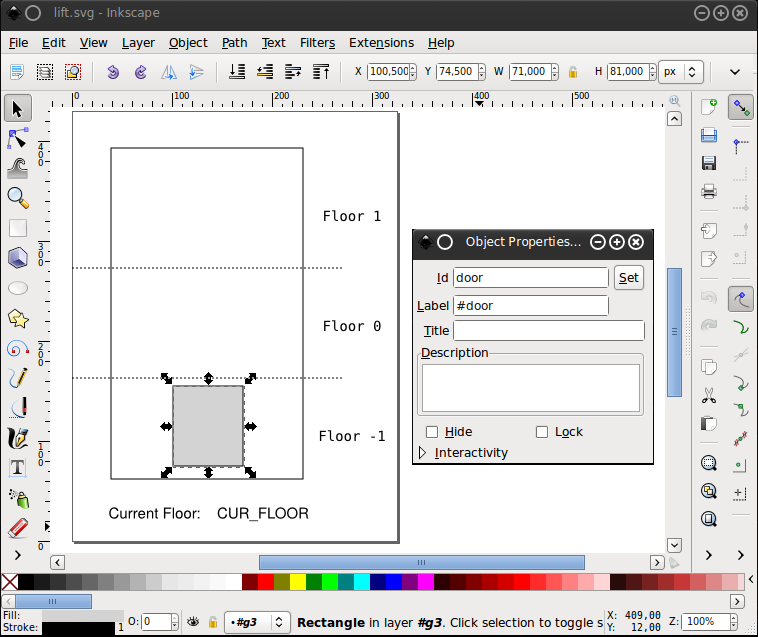
\includegraphics[width=12cm]{img/tutorial/tut_02.png}
	\caption{Creating an SVG graphic with Inkscape}
	\label{fig_tut_02_inkscape}
\end{center}
\end{figure}

%Please download the prepared \file{lift.svg}{lift.svg} file and put it relative to your \texttt{template.html} file in your workspace.
%Add the following tag within the body tag in your \texttt{template.html} file:
%\begin{lstlisting}[language=html]
%<object data="lift.svg" type="image/svg+xml" data-bms="svg">
%</object>
%\end{lstlisting}

Please download the prepared \file{lift.svg}{lift.svg} file and open it with Inkscape as demonstrated in Figure~\ref{fig_tut_02_inkscape}.
Feel free to modify and explore the SVG graphic.
In order to link visual elements of the SVG graphic with the formal model, we have to give them identifiers. 
For this, select an element, open the context menu and select \textsf{Object Properties}.
A popup window should be opened as demonstrated in Figure~\ref{fig_tut_02_inkscape}.
As an example, we give the visual element that represents the door, the id ``door''.
In Section~\ref{sec_creation_observers} we explain how we can use this information in order to create the link between the formal model and the visualisation by means of observers.
If you are satisfied with your SVG graphic, save it as a plain SVG graphic with \textsf{File $\rangle$ Save As}.
Select \textsf{Plan SVG (*.svg)} as an output format and click on the \textsf{Save} button.
You can save the SVG file anywhere on your local system. 
Open the SVG file with a text editor of your choice and put the SVG code within the body tag in the \texttt{template.html} file located in your workspace.
